%-----------------------------------------------------------------------------
%
%               Template for sigplanconf LaTeX Class
%
% Name:         sigplanconf-template.tex
%
% Purpose:      A template for sigplanconf.cls, which is a LaTeX 2e class
%               file for SIGPLAN conference proceedings.
%
% Guide:        Refer to "Author's Guide to the ACM SIGPLAN Class,"
%               sigplanconf-guide.pdf
%
% Author:       Paul C. Anagnostopoulos
%               Windfall Software
%               978 371-2316
%               paul@windfall.com
%
% Created:      15 February 2005
%
%-----------------------------------------------------------------------------


\documentclass[pldi]{sigplanconf}

% The following \documentclass options may be useful:

% preprint      Remove this option only once the paper is in final form.
% 10pt          To set in 10-point type instead of 9-point.
% 11pt          To set in 11-point type instead of 9-point.
% authoryear    To obtain author/year citation style instead of numeric.

\usepackage{courier}            % standard fixed width font
\usepackage[scaled]{helvet} % see www.ctan.org/get/macros/latex/required/psnfss/psnfss2e.pdf
\usepackage{listings}          % format code
\usepackage{enumitem}      % adjust spacing in enums
\usepackage{xspace}
\usepackage{mathtools}
\usepackage{mathpartir}
\usepackage{amssymb}
\usepackage{amsmath}
\usepackage{latexsym}
\usepackage{graphicx}
\usepackage[usenames,dvipsnames]{color}
\usepackage{listings}
\usepackage{subcaption}
\usepackage{stmaryrd}
\usepackage{comment}
\usepackage{float}
\usepackage{verbatimbox}
\usepackage{breakurl}
\usepackage[breaklinks]{hyperref}

%Formatting Commands
%-------------------
\newcommand{\C}[1]{\code{#1}}
\renewcommand{\k}[1]{\mathtt{#1}} % Code font in math mode.
\newcommand{\code}[1]{\,{\tt #1}\,}
\newcommand{\conj}{\wedge}
\newcommand{\disj}{\vee}
\newcommand{\seqn}[1]{\overline {#1}}
\newcommand{\tuplee}[1]{\langle #1 \rangle}
\newcommand{\ALT}{~\mid~}
\newcommand{\lamb}[2]{\lambda #1.\,#2}
\newcommand{\spc}[0]{\quad}
\newcommand{\U}[0]{\cup}
\newcommand{\X}[0]{\times}
\newcommand{\xn}[0]{\cap}
\newcommand{\redsto}[0]{\longrightarrow}
\newcommand{\rredsto}[0]{\rightsquigarrow_r }
\newcommand{\evalsto}[0]{\longrightarrow }
\newcommand{\env}[0]{\Gamma}
\newcommand{\finmaparrow}[0]{\overset { Fin }{ \longrightarrow } }
\newcommand{\envwf}[1]{\vdash\,#1}
\newcommand{\tywf}[2]{#1\,\vdash\,#2 \; \texttt{ok}}
\newcommand{\fgjtywf}[2]{#1\,\Vdash\,#2 \; \texttt{ok}}
\newcommand{\isvalid}[2]{#1\,\vdash\,#2}
\newcommand{\hastyp}[3]{#1\,\vdash\,#2:#3}
\newcommand{\hasfgjtyp}[3]{#1\,\Vdash^{}\,#2\,:\,#3}
\newcommand{\hassort}[3]{#1\,\vdash\,#2\,::\,#3}
\newcommand{\subtyp}[3]{#1\,\vdash\,#2 <: #3}
\newcommand{\fgjsubtyp}[3]{#1\,\Vdash\,#2 <: #3}
\newcommand{\generalizes}[3]{#1\,\vdash\,#2 \succ #3}
\newcommand{\msfolsig}[0]{{\Lambda \equiv}}
%\newcommand{\msentails}[2]{#1\,\models_L\,#2}
\newcommand{\msentails}[2]{#1\,\models\,#2}
\newcommand{\thesemof}[1]{ \llbracket #1 \rrbracket}
\newcommand{\defeq}[0]{ \triangleq }
\newcommand{\tymap}[0]{\mathcal{F}}
\newcommand{\etaeq}[0]{\eta_{eq}}
\newcommand{\semof}[1]{\thesemof{#1}}
\newcommand{\mssemof}[1]{\thesemof{#1}}
\newcommand{\rwsto}[0]{=}
\newcommand{\rrwsto}[0]{\hookrightarrow}
\newcommand{\rwbindfwd}[0]{\gamma_{\Rightarrow}}
\newcommand{\rwbindbwd}[0]{\gamma_{\Leftarrow}}
\newcommand{\eqhlt}[1]{\underline{#1}}
\newcommand{\tfr}[0]{F_R}
\newcommand{\ground}[1]{\underline{#1}}
\newcommand{\semeq}[0]{\equiv}
\newcommand{\elabsto}[0]{\looparrowright }
\newcommand{\arr}[0]{$\rightarrow$}
\newcommand{\eef}[0]{$\Leftrightarrow$}
\newcommand{\imp}[0]{$\Rightarrow$}
\newcommand{\RNull}[0]{\emptyset}
\newcommand{\cty}[0]{ty}
\newcommand{\hsp}[0]{\hspace*{-0.1in}}
\newcommand{\hspa}[0]{\hspace*{-0.08in}}
% removable:
\newcommand{\subst}[2]{\lbrack #1/#2 \rbrack}
\newcommand{\absof}[1]{\left\| #1 \right\| }
\newcommand{\broom}{{\sc Broom}\xspace}
\newcommand{\name}{{\sc Broom}\xspace}
\newcommand{\fbname}{{\sc Featherweight Broom}\xspace}
\newcommand{\FB}{{\sc FB}\xspace}
\newcommand{\naiad}{{\sc Naiad}\xspace}
\newcommand{\csolve}{{\sc Csolve}\xspace}
\newcommand{\GK}[1]{{\textcolor{red}{{GK: #1}}}}
\newcommand{\csharp}{C\#~}
\newcommand{\outlives}{\succeq}
\newcommand{\coloneqq}{::=}
\newcommand{\R}[1]{\textrm{#1}}
\newcommand{\N}[1]{{\normalfont #1}}
\newcommand{\M}[1]{\mathtt{#1}}
\newcommand{\ObjZ}{\C{Object}}
\newcommand{\RgnZ}{\C{Region}}
\newcommand{\thisZ}{\C{this}}
\newcommand{\superZ}{\C{super}}
\newcommand{\unitZ}{\C{unit}}
\newcommand{\FuncZ}{\C{Func}}
\newcommand{\unitval}{\C{()}}
\newcommand{\inang}[1]{\langle #1 \rangle}
\newcommand{\rhoalloc}{\rho^a}
\newcommand{\rhobar}{\bar{\rho}}
\newcommand{\rhoallocm}{\rho^a_m}
\newcommand{\rhobarm}{\bar{\rho_m}}
\newcommand{\ralloc}{\pi^a}
\newcommand{\rgn}{\pi}
\newcommand{\rbar}{\bar{\pi}}
\newcommand{\tbar}{\bar{T}}
\newcommand{\taubar}{\bar{\tau}}
\newcommand{\xbar}{\bar{x}}
\newcommand{\vbar}{\bar{v}}
\newcommand{\ebar}{\bar{e}}
\newcommand{\extends}{\triangleleft}
\newcommand{\rextends}{\blacktriangleleft}
\renewcommand{\bar}[1]{\overline{#1}}
\newcommand{\angR}{\inang{\rhoalloc\rhobar \,|\, \phi}}
\newcommand{\angT}{\inang{\tbar}}
\newcommand{\tyvar}{a}
\newcommand{\tyvarb}{b}
\newcommand{\angAlpha}{\inang{\bar{\tyvar} \extends \bar{\fgjN}}}
\newcommand{\fgjN}{K}
\newcommand{\fbN}{N}
\newcommand{\headerOf}[1]{\C{class}\; #1\angR\angAlpha \extends \fbN}
\newcommand{\substFn}{\mathcal{S}}
\newcommand{\mang}{\inang{\rhoalloc_m\bar{\rho_m} \,|\, \phi_m}}
\newcommand{\rhoset}{\Sigma}
\newcommand{\rhoenv}{\Delta}
\newcommand{\aenv}{\Theta}
\newcommand{\phicx}{\Phi}
\newcommand{\subtypcx}{\rhoset,\rhoenv,\aenv,\phicx}
\newcommand{\A}{{\mathcal{A}}}
\newcommand{\exptycx}[2]{\A,#1,#2}
\newcommand{\void}{\C{void}}
\newcommand{\functy}[3]{\FuncZ\inang{#1}\inang{#2,#3}}
\newcommand{\stmtsemcx}{\A,\env}
\newcommand{\stmtsemcxp}{\A',\env'}
\newcommand{\stmtsemcxpp}{\A'',\env''}
\newcommand{\sredsto}{\Rightarrow}
\newcommand{\stmtsem}[4]{#1 \, \vdash \, #2 \,/\, #3 \sredsto #4}
\newcommand{\okin}[2]{#1 \; \texttt{ok} \; \texttt{in} \; #2}
\newcommand{\lambdaexp}[3]{\lambda\inang{#1}(#2) \Rightarrow #3}
\newcommand{\Lambdaexp}[2]{\Lambda\inang{#1}.#2}
\newcommand{\letexp}[3]{\C{let}\;#1\,=\,#2\;\C{in}\;#3}
\newcommand{\letregion}[2]{\C{letregion}\;#1\;\C{in}\;#2}
\newcommand{\open}[3]{\C{open}\;#1\;\C{withroot}\;#2\;\C{in}\;#3}
\newcommand{\openalloc}[3]{\C{openalloc}\;#1\;\C{withroot}\;#2\;\C{in}\;#3}
\newcommand{\unpackexp}[4]{\C{let}\;(#1,\,#2)\,=\,\C{unpack}\;#3\;\C{in}\;#4}

%Rules
%-----
\newcommand{\rulelabel}[1]{\textrm{\sc {#1}}}
\newcommand{\ilrulelabel}[1]{{\sc #1}}
\newcommand{\RULE}[2]{\frac{\begin{array}{c}#1\end{array}}
                           {\begin{array}{c}#2\end{array}}}

% Math mode
%-----------
\newenvironment{nop}{}{}
\newenvironment{smathpar}{
\begin{nop}\small\begin{mathpar}}{
\end{mathpar}\end{nop}\ignorespacesafterend}

% Theorems Environment
%----------------------
\newtheorem{theorem}{Theorem}[section]
\newtheorem{lemma}[theorem]{Lemma}
\newtheorem{proposition}[theorem]{Proposition}
\newtheorem{corollary}[theorem]{Corollary}

\newenvironment{proof}[1][Proof]{\begin{trivlist}
\item[\hskip \labelsep {\bfseries #1}]}{\end{trivlist}}
\newenvironment{definition}[1][Definition]{\begin{trivlist}
\item[\hskip \labelsep {\bfseries #1}]}{\end{trivlist}}
\newenvironment{example}[1][Example]{\begin{trivlist}
\item[\hskip \labelsep {\bfseries #1}]}{\end{trivlist}}
\newenvironment{remark}[1][Remark]{\begin{trivlist}
\item[\hskip \labelsep {\bfseries #1}]}{\end{trivlist}}

\newcommand{\qed}{\nobreak \ifvmode \relax \else
      \ifdim\lastskip<1.5em \hskip-\lastskip
      \hskip1.5em plus0em minus0.5em \fi \nobreak
      \vrule height0.75em width0.5em depth0.25em\fi}

\usepackage{listings}
\usepackage{subcaption}
\usepackage{stmaryrd}
\usepackage[skip=5pt]{caption}

\newcommand{\lstjava}{\lstset{ %
language=Java, % choose the language of the code
basicstyle=\small\ttfamily,       % the size of the fonts that are used for the code
keywordstyle=\color{Bittersweet},
% numbers=left,                   % where to put the line-numbers
numberstyle=\tiny,      % the size of the fonts that are used for the line-numbers
stepnumber=1,                   % the step between two line-numbers. If it is 1 each line will be numbered
numbersep=5pt,                  % how far the line-numbers are from the code
showspaces=false,               % show spaces adding particular underscores
showstringspaces=false,         % underline spaces within strings
showtabs=false,                 % show tabs within strings adding particular underscores
% frame=single,                   % adds a frame around the code
tabsize=2,                      % sets default tabsize to 2 spaces
captionpos=b,                   % sets the caption-position to bottom
breaklines=true,                % sets automatic line breaking
breakatwhitespace=false,        % sets if automatic breaks should only happen at whitespace
commentstyle=\itshape\color{MidnightBlue},
%escapeinside={\%*}{*)},         % if you want to add a comment within your code
morekeywords={letregion, let, in, openalloc, open, withroot, not, : , /\\}
}}
\lstnewenvironment{codejava}
    { % \centering
			\lstjava
      \lstset{mathescape=true}%
      \csname lst@setfirstlabel\endcsname}
    { %\centering
      \csname lst@savefirstlabel\endcsname}

\lstnewenvironment{numcodejava}
    { % \centering
			\lstjava
      \lstset{numbers=left,firstnumber=1}%
      \csname lst@setfirstlabel\endcsname}
    { %\centering
      \csname lst@savefirstlabel\endcsname}


\begin{document}

% Uncomment one of the following two, if you are not going for the 
% traditional copyright transfer agreement.

%\exclusivelicense                % ACM gets exclusive license to publish, 
                                  % you retain copyright

%\permissiontopublish             % ACM gets nonexclusive license to publish
                                  % (paid open-access papers, 
                                  % short abstracts)

% \titlebanner{banner above paper title}        % These are ignored unless
% \preprintfooter{short description of paper}   % 'preprint' option specified.

%The Paper
%---------------------
\title{Broom: Safe Region-Based Memory Management for Dataflow
Programs}

\authorinfo{}
           {}
           {}
\maketitle

\begin{abstract}

Distributed execution engines, such as MapReduce and Dryad, represent
a data-parallel computation as a dataflow graph with computational
vertices connected by communication edges. The computation is run by
executing the vertices of this graph on a set of available computers,
while communication edges are materialized as either network
connections, or appropriate inter-process communication channels.
Although MapReduce and Dryad can perform optimal distribution the
computation across available computers, they nevertheless rely on
language runtimes, such as JVM or C\#.Net, to manage an atomic
computation on a given machine. 

In this paper, we demonstrate that the general purpose garbage
collection scheme employed by C\#.Net runtime is not very effective
for dataflow programs to the extent that the latency due to GC is
intolerably high in many practical examples. We propose a memory
management scheme that combines user-managed memory regions with
automatic garbage collection, and lets programmers exploit specific
memory behaviours exhibited by dataflow programs. To protect
programmers from the dangers of manual memory management, we
supplement our memory management scheme with a region type system that
statically ensures the memory safety of region-annotated C\# programs,
even in presence of higher-order stateful functions. Further, we
describe a type inference algorithm that infers principal region types
for first-order programs thereby saving programmers the need to write
region annotations on types. Our inference algorithm is also very
effective, albeit incomplete, for higher-order programs. As a
testament to efficacy of our approach, we demonstrate performance
improvements over a range of realistic dataflow programs that were
rewritten to use region-based manual memory management, but are
nevertheless judged to be safe by our type system.

\end{abstract}

% general terms are not compulsory anymore, 
% you may leave them out
%% \terms
%% term1, term2

\newcommand{\TODO}[1]{\textbf{TODO: #1}} \newcommand{\eg}{\emph{e.g.}}
\newcommand{\ie}{\emph{i.e.}}

\section{Introduction} \label{sec:introduction}

In this paper, we present a \emph{safe} and \emph{efficient} region-based approach
to \emph{transferring data} between a set of concurrent actors, motivated by the following concerns.

Consider the example (of  a producer creating a data structure and transferring it to a consumer)
in Fig.~\ref{fig:motivating-eg}. This represents a \C{SELECT} query operator for streaming data. 
The operator receives a stream of input messages, each
associated with a time (window) $t$, processed by method
\texttt{onReceive}.  Each input message contains a list of inputs,
each of which is processed by applying a user-defined function to
create a corresponding output.  The operator may receive multiple
messages with the same timestamp (and messages with different
timestamps may be delivered out of order). A timing-message (an
invocation of method \texttt{OnNotify}) indicates that no more input
messages with a timestamp $t$ will be subsequently delivered.  At this
point, the operator completes the processing for time window $t$ and
sends a corresponding output message to its successor.

\begin{figure}[t!]
\begin{numcodejava}
class MapVertex<TIn, TOut> {
  Func<TIn, TOut> selector;
  Dictionary<Time, List<TOut>> map;
  ...
  void onReceive(Time t, List<TIn> inputs) {
    if (!map.ContainsKey(t))
       map[t] = new List<TOut>();
    foreach (TIn input in inputs) {
      TOut output = selector(input);
      map[t].add(output);
    }
  }
  void onNotify(Time t) {
     List<TOut> outputList = map[t];
     map.Remove(t);
     transfer(successorId, t, outputList); 
  }
}
\end{numcodejava}
\caption{\C{SELECT} dataflow operator}
\label{fig:motivating-eg}
\end{figure}



\paragraph{Performance.}
When the transferred data structures are large, as is the case with many streaming big-data
analysis systems, garbage collection overhead becomes
significant~\cite{Broom:HotOS}.  Furthermore, in a distributed
dataflow system, the GC pause at one node can have a cascading adverse
effect on the performance of other nodes~\cite{Broom:HotOS,harris15}:
a GC pause at an upstream actor can block downstream actors that are waiting for
messages.  However, often much of the GC overhead results from the
collector performing avoidable or unproductive work.  For the example
in Fig.~\ref{fig:motivating-eg}, GC might repeatedly traverse the
\C{map} data structure, although its objects cannot be collected until a
suitable timing message arrives.


\begin{figure}
\centering
\subcaptionbox {
  Before transfer.
  \label{fig:after-transfer}
} [
  0.35\columnwidth
] {
  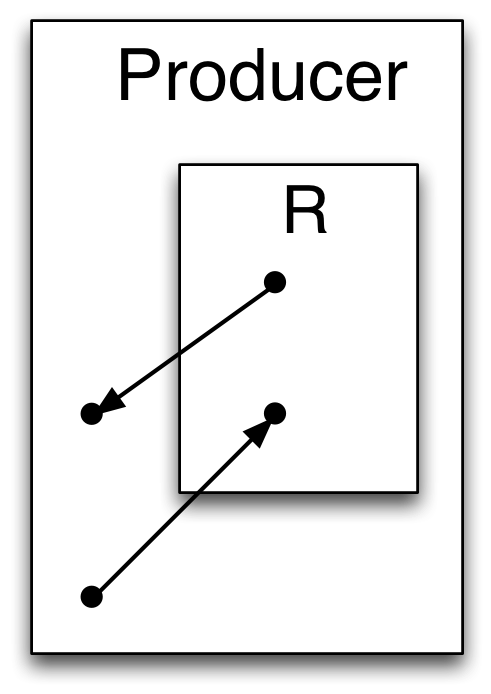
\includegraphics[scale=0.36]{producer-heap}
}
\subcaptionbox {
  After transfer.
  \label{fig:before-transfer}
} {
  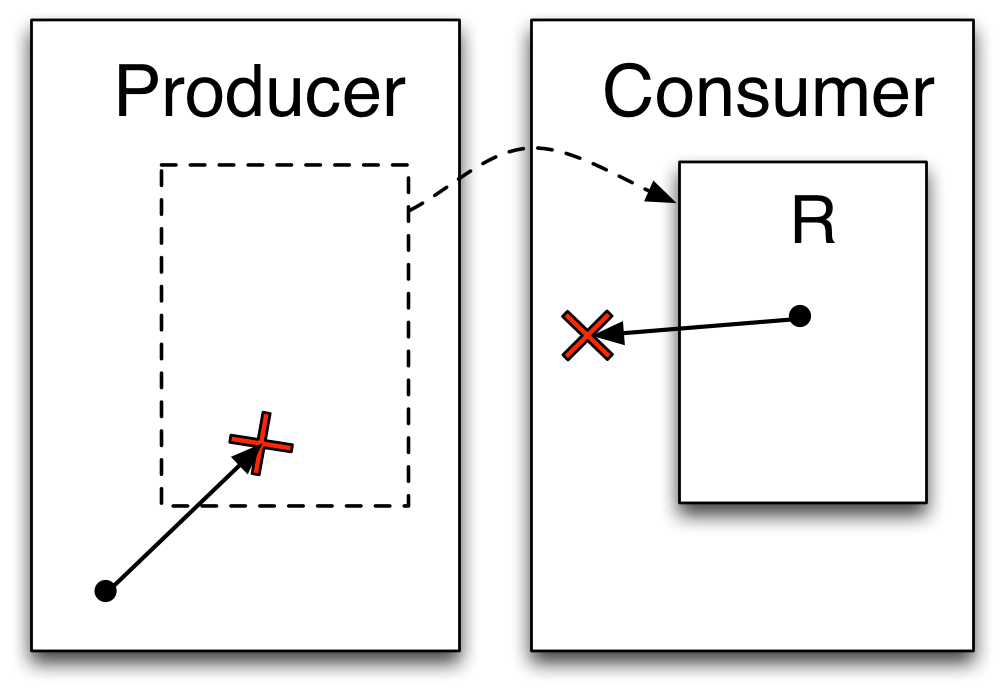
\includegraphics[scale=0.36]{producer-consumer-heap}
}

\caption{References in and out of a transferable region ($R$) become
invalid after transfer.}
\label{fig:transfer-violations}
\end{figure}

\paragraph{Safety.}
These systems are designed to allow the producer and consumer to
execute in the same address space or in different address spaces
(as determined by the compiler and runtime).
We wish to ensure memory safety in the presence of such transferred data by ensuring
that there are no invalid references. A transfer operation, with no
additional checks, may cause memory safety violations, both at the
producer of the data structure, and its (possibly remote) consumer. At
the producer, any existing references into the transferred data structure become
invalid post transfer. If the data structure contains references to
objects outside (the transferred data), then such references become
invalid in the context of the consumer. Both scenarios are depicted in
Fig.~\ref{fig:transfer-violations}. Safety violations of this kind are
particularly unwelcome in the context of languages like C\# and Java
that are otherwise memory-safe. While references from within the
transferable data to outside can be disallowed in the interest of safety,
references into transferable data needs to be allowed before the data
is transferred. Allowing such references is crucial to performance,
as any non-trivial program creates temporary references to the internal
objects of a data-structure.

\paragraph{Safe Transferable Regions.}
In this paper, we present a language-based approach to safely and
efficiently realize such transferable data that uses regions as
the implementation technique.
%
A region is a block of memory that is allocated
and freed in one shot, often in constant time. A region may contain
one or more contiguous range of memory locations, and individual
objects may be dynamically allocated within the region over time,
while they are deallocated en masse when the region is freed.  Thus, a
region is a good fit for a transferable data-structure.  In
Fig.~\ref{fig:motivating-eg}, the output to be constructed for each
time window $t$ (i.e., \C{map[t]}) can be a separate region that is
allocated when the first message with timestamp $t$ arrives, and
deallocated after \C{map[t]} is transferred in \C{onNotify}.

The use of regions alleviates the performance concern related to
garbage collection described earlier.
However, manual region memory management introduces memory safety
issues such as dangling pointers.
We present a single type system that simultaneously addresses
this safety concern, as well as those described above related to
the use of \emph{transferable data}.

% Region-based memory management, both manual as well as automatic, has
% been known for a long time. Manual region-based memory management
% suffers from the usual drawbacks, namely the potential for invalid
% references and the consequent lack of memory safety. Automatic
% region-based memory management systems guarantee memory safety, but
% impose various restrictions.  MLKit, which implements the approach
Safe region-based memory management using types was
pioneered by Tofte and Talpin~\cite{tofte94,tofte97}, who 
use only lexically scoped regions.  At runtime, the set of all regions
(existing at a point in time) forms a stack. Thus, the lifetimes of
all regions must be well-nested: it is not possible to have two
regions whose lifetimes overlap, with neither one's lifetime contained
within the other.  Unfortunately, the data structures in the above
example do not satisfy this restriction (as the output messages for
multiple time windows may be simultaneously live, without any
containment relation between their lifetimes).  We refer to regions
with lexically scoped lifetimes as \emph{stack regions} and to regions
that do not have such a lexically scoped region as \emph{dynamic}
regions.

Our focus, in this paper, is on first-class \emph{memory-safe} dynamic regions
that can be safely transferred across address spaces. We refer to such dynamic
regions as \emph{transferable} regions.
%
Our approach is based on a variation of ideas introduced by~\cite{WW01,cyclone04}
that combine linear types and regions to suport dynamic regions.
Unlike the prior work, we ensure memory safety in the presence of
transferable regions through a \emph{combination of a static
typing discipline and lightweight runtime checks in place of linear types}.

The cornerstone of this approach is an \C{open} lexical block for transferable regions,
that ``opens'' a transferable region and guarantees that the region
won't be transferred/freed while it is open. By nesting an
MLKit-style \C{letregion} lexical block, that delimits
the lifetime of a stack region, inside an \C{open} lexical block for a
transferable region, we can guarantee that the transferable region
will remain live as long as the stack region is live. We say that the
former \emph{outlives} the later., and any references from the stack
region to the transferable region are therefore safe.  Next, we note
that by controlling the outlives relationships between various
regions, we only allow safe cross-region references, while prohibiting
unsafe ones. In the above example, an outlives relationship
\emph{from} the stack region \emph{to} the transferable region means
that the references in that direction are allowed, but not the
references in the opposite direction. In contrast, if an \C{open}
block of a transferable region $R_0$ is nested inside an \C{open}
block of another transferable region $R_1$, we do not establish any
outlives relationships, thus declaring our intention to not allow any
cross-region references between $R_0$ and $R_1$.  Finally, we observe
that outlives relationships are established based on the lexical
structure of the program, hence a static type system can enforce them
effectively. By assigning region types to objects, which capture the
regions such objects are allocated in, and by maintaining outlives
relationships between various regions, we can statically decide the
safety of all references in the program.

Ensuring memory safety using this approach requires ensuring
that the use of transferable regions satisfies certain temporal properties.
Firstly, a transferable region should not be transferred/freed
inside an open block of that region (i.e, while it is still open).
Secondly, a transferred/freed region should not be opened. These are
typestate invariants on the transferable region objects, which are
hard to enforce statically in the presence of unrestricted
aliasing. Techniques like linear types and unique pointers can be used
to restrict aliasing, but the constraints they impose are often hard
to program around. We therefore enforce typestate invariants at
runtime via lightweight checks. In particular, we define an acceptable
state transition discipline for transferable regions
(Fig.~\ref{fig:region-fsm}), and check, at runtime, whether a given
transition of a transferable region (\eg, from \emph{open} state to
\emph{freed} state) is valid or not. The check is lightweight since it
only involves checking a single tag that captures the current state.
We believe that this is a reasonable choice since regions are
coarse-grained objects manipulated infrequently, when compared to the
fine-grained objects that are present inside these regions, for which
safety is enforced statically. 

One of the novel contributions of this paper is a type inference algorithm
that eliminates the need for users to write region type annotations.
This, we believe, significantly reduces the impediment to adopt our
approach in practical setting.


% transferableally checking for the second category of
% invariants is easy and does not pose a performance concern (unlike,
% \eg, the first category of constraints); a static typechecker that
% rules out the second category of violations would be very restrictive
% from an expressiveness perspective; finally, the human effort required
% to ensure the second set of invariants is not as burdensome (as
% regions are coarse-grained objects manipulated infrequently), \eg, as
% it would be for the first set of invariants.

% when a producer transfers a
% region containing a data structure to a consumer, in a shared-memory
% context, we enforce an ownership discipline that ensures that the
% producer cannot subsequently modify the data structure. When the same
% transfer happens in a distributed setting, we guarantee that (a). the
% data structure is contained in the region, and can be safely
% transmitted across address spaces, and (b). once the transfer
% concludes, the producer can safely deallocate the memory for the
% data structure without the fear of violating memory safety.

%  Transfer operation,
% with no additional checks and balances, may cause memory safety
% violations, both at the producer of the data structure, and the
% (possibly remote) consumer of the data structure. A key invariant and restriction
% that we utilize
% to achieve this is that no object $o_1$ in one transferable region $D_1$
% can contain a pointer to an object $o_2$ in another transferable region
% $D_2$.  In cases where this is too restrictive, the user has to resort
% to (deep) copying $o_2$ to $D_1$.  This is conceptually quite
% reasonable given the perspective that $D_1$ is a self-contained
% data structure.  Furthermore, this is quite analogous, from a
% performance perspective, to the copying that happens when a garbage
% collector promotes an object from a lower generation to a higher
% generation.  From this perspective, a region may be seen as a
% user-controlled generation.

% This ensures that we can safely free one transferable region (\eg, the
% input-message in our example) without affecting the validity of
% pointers in another transferable region (\eg, the output-message).
% However, this is not sufficient! When processing the input-message
% $D$, we necessarily will have to create pointers that point to objects
% that are internal to $D$. Such pointers may be stack-allocated or even
% reside in the heap (\eg, consider the iterator object used to iterate
% over the list in the input-message).  How do we ensure the safety of
% these pointers?

% We use \emph{stack regions} (regions with lexically-scoped lifetimes),
% as well as the stack, for such temporary pointers (to objects inside a
% transferable region) and use the following protocol to ensure safety
% of such pointers.  To work with a transferable region $D$, we must
% first \emph{open} the region $D$, to indicate that $D$ should not be
% freed during this period. When the processing of the region is
% complete, we \emph{close} the region $D$, to indicate that it is safe
% to free $D$.  In general, a transferable region may be opened and
% closed multiple times before it is eventually transferred or freed.

% Our type-system permits the creation of pointers to internal objects
% of \emph{open transferable} regions, but uses lexical scoping to ensure
% that such pointers are no longer live when the region is closed.
% Thus, such pointers may be either stack-allocated or reside in a
% region whose lifetime is statically guaranteed to be contained within
% the interval when $D$ is open.  As a consequence, the system ensures
% the strong invariant that for a \emph{closed transferable} region $D$ no
% pointer from outside $D$ points to an internal object of $D$.

% The final piece required to ensure memory-safety is ensuring that the
% program correctly follows the above-mentioned protocol for transferable
% regions: \eg, an open region should not be freed and, dually, a freed
% region should not be opened.  (A complete typestate specification of
% the protocol is presented later.)

% Transferable regions are first-class objects in our system. For instance,
% in our running example, we would like to use a dictionary that stores
% transferable regions. However, this means that the program may create
% multiple aliases (pointers) to the same region, which, in turn, means
% that statically checking if the program correctly follows the transferable
% region protocol is hard (undecidable, in fact). Safety can be ensured
% by using, \eg, linear typing to prevent the creation of aliases, but
% this would be quite restrictive. Hence, in our system, we transferableally
% check for adherence to this protocol.

% In summary, our approach reduces memory safety to two sub-problems:
% (a) Ensuring  low-level invariants about pointers to (fine-grained)
% objects inside regions and (b) Ensuring higher-level (typestate)
% invariants about the regions themselves.  We use a type system to
% statically ensure the first set of invariants. We use a transferable check
% to ensure that the second set of invariants are satisfied at runtime.
% %
% This is a novel aspect of our system. We believe that this is a
% reasonable choice: transferableally checking for the second category of
% invariants is easy and does not pose a performance concern (unlike,
% \eg, the first category of constraints); a static typechecker that
% rules out the second category of violations would be very restrictive
% from an expressiveness perspective; finally, the human effort required
% to ensure the second set of invariants is not as burdensome (as
% regions are coarse-grained objects manipulated infrequently), \eg, as
% it would be for the first set of invariants.
% =======
% objects. Though we focus, in this paper, on memory-safety, our
% approach offers other benefits.  When a producer transfers a
% data-structure to a consumer, in a shared-memory context , our
% approach provides an ownership discipline that ensures that the
% producer cannot subsequently modify the data-structure. When the same
% transfer happens in a distributed setting, the system guarantees that
% the data-structure is self-contained and can be safely transmitted
% across address spaces.  We refer to dynamic regions that provide these
% guarantees as \emph{transferable} regions.

% The key memory safety property we wish to ensure is that there are no
% dangling references: i.e., a reference to an object that has been
% freed.  A key invariant and restriction that we utilize to achieve
% this is that no object $o_1$ in one dynamic region $D_1$ can contain a
% pointer to an object $o_2$ in another dynamic region $D_2$.  In cases
% where this is too restrictive, the user has to resort to (deep)
% copying $o_2$ to $D_1$.  This is conceptually quite reasonable given
% the perspective that $D_1$ is a self-contained data-structure.
% Furthermore, this is quite analogous, from a performance perspective,
% to the copying that happens when a garbage collector promotes an
% object from a lower generation to a higher generation.  From this
% perspective, a region may be seen as a user-controlled generation.

% This ensures that we can safely free one dynamic region (\eg, the
% input-message in our example) without affecting the validity of
% pointers in another dynamic region (\eg, the output-message).
% However, this is not sufficient! \dv{for what} When processing the input-message
% $D$, we necessarily will have to create pointers that point to objects
% that are internal to $D$. Such pointers may be stack-allocated or even
% reside in the heap (\eg, consider the iterator object used to iterate
% over the list in the input-message).  How do we ensure the safety of
% these pointers?

% We use \emph{stack regions} (regions with lexically-scoped lifetimes),
% as well as the stack, for such temporary pointers (to objects inside a
% dynamic region) and use the following protocol to ensure safety of
% such pointers.  To work with a dynamic region $D$, we must first
% \emph{open} region $D$, to indicate that $D$ should not be freed
% during this period.  When the processing of the region is complete, we
% \emph{close} the region $D$, to indicate that it is safe to free $D$.
% In general, a dynamic region may be opened and closed multiple times
% before it is finally freed.

% Our type-system permits the creation of pointers to internal objects
% of \emph{open dynamic} regions, but uses lexical scoping to ensure
% that such pointers are no longer live when the region is closed.
% Thus, such pointers may be either stack-allocated or reside in a
% region whose lifetime is statically guaranteed to be contained within
% the interval when $D$ is open.  As a consequence, the system ensures
% the strong invariant that for a \emph{closed dynamic} region $D$ no
% pointer from outside $D$ points to an internal object of $D$.

% The final piece required to ensure memory-safety is ensuring that the
% program correctly follows the above-mentioned protocol for dynamic
% regions: \eg, an open region should not be freed and, dually, a freed
% region should not be opened.  (A complete typestate specification of
% the protocol is presented later.)

% Dynamic regions are first-class objects in our system. For instance,
% in our running example, we would like to use a dictionary that stores
% dynamic regions. However, this means that the program may create
% multiple aliases (pointers) to the same region, which, in turn, means
% that statically checking if the program correctly follows the dynamic
% region protocol is hard (undecidable, in fact). Safety can be ensured
% by using, \eg, linear typing to prevent the creation of aliases, but
% this would be quite restrictive. Hence, in our system, we dynamically
% check for adherence to this protocol.

% In summary, our approach reduces memory safety to two sub-problems:
% (a) Ensuring  low-level invariants about pointers to (fine-grained)
% objects inside regions and (b) Ensuring higher-level (typestate)
% invariants about the regions themselves.  We use a type system to
% statically ensure the first set of invariants. We use a dynamic check
% to ensure that the second set of invariants are satisfied at runtime.
% %
% This is a novel aspect of our system. We believe that this is a
% reasonable choice: dynamically checking for the second category of
% invariants is easy and does not pose a performance concern (unlike,
% \eg, the first category of constraints); a static typechecker that
% rules out the second category of violations would be very restrictive
% from an expressiveness perspective; finally, the human effort required
% to ensure the second set of invariants is not as burdensome (as
% regions are coarse-grained objects manipulated infrequently), \eg, as
% it would be for the first set of invariants.
% >>>>>>> af17b22a358a6165ae10628a5247cd4fa66adc07

\subsection*{Contributions}

The paper makes the following contributions:

\begin{itemize} 
  \item We present \name, a \csharp-like typed
  object-oriented language that eschews garbage collection in favour of
  programmer-managed memory regions . \name extends its core language,
  which includes \emph{lambdas} (higher-order functions) and
  \emph{generics} (parametric polymorphism), with constructs to create,
  manage and destroy static and transferable memory regions. Transferable regions
  are first-class values in \name.
  % Experiments demonstrate that   \naiad~\cite{naiad} dataflow
  % program using programmer-managed memory regions outperform their
  % GC counterparts by a margin of upto 59\%. 

  \item \name is equipped with a region type system that statically
  guarantees safety of all memory accesses in a well-typed program,
  provided that certain typestate invariants on regions hold.  The
  later invariants are enforced via simple runtime checks.
% The correctness of region usage is checked efficiently at run-time.
% The overhead of checking these conditions is less than \GK{x\%} in
% our experiments with \naiad workloads.

  \item We define an operational semantics for \name, and a type
  safety result that clearly defines and proves safety guarantees
  described above.

  \item We describe a region type inference algorithm for \name that
  (a). completely eliminates the need to annotate \name programs with
  region types, and (b). enables seamless interoperability between
  region-aware \name programs and legacy standard library code that is
  region-oblivious. The cornerstone of our inference algorithm is a
  novel constraint solver that performs abduction in a partial-order
  constraint domain to infer weakest solutions to recursive
  constraints.

  \item We describe an implementation of \name frontend in OCaml,
  along with case studies where the region type system was able to
  identify unsafe memory accesses statically.
  
\end{itemize}

  %The rest of the paper is organized as follows. The next section
  %presents an informal overview of \name, and motivates the need for a
  %region type system.  \S~\ref{sec:type-system} formalizes the type
  %system and its safety guarantees. The type inference algorithm is
  %described in \S~\ref{sec:type-inference}. \S~\ref{sec:csolve} focuses
  %on \csolve, the constraint solving algorithm, and its correctness
  %guarantees.  Implementations details and practical extensions to the
  %type system are described in \S~\ref{sec:implementation}.
  %\S~\ref{sec:evaluation} presents experimental evaluation and case
  %studies.  \S~\ref{sec:related} discusses the related work, and
  %\S~\ref{sec:conclusion} concludes.

% , and it is undesirable to allocate them in a transferable
% region; such regions are meant for the data being transferred.

\textbf{TO DO:}

As with allocation and deallocation, transferring a memory region is fast, and therefore,
transferring a data structure contained in a region is more efficient
that traversing its objects in heap, and transferring them
independently.
In the \C{SelectVertex} example from
Fig.~\ref{fig:motivating-eg}, the proposed region to contain the
output for each time window $t$ must be transferable due to the
\C{transfer} operation on Line 16. As it is the case with
\C{SelectVertex}, the transferred data is no longer accessed by the
producer, so the transfer operation in our system deallocates the
region once the transfer is complete.

Since transferable regions are first class objects in our setting,
controlling references to and from such regions while ensuring their
safety without significantly diluting the performance advantage of
regions over GC is a challenging exercise.

An important observation, in the context of processes of the kind
described above, is that the data-structures exchanged between them
can be partitioned into sets of fate-sharing objects with common
lifetimes, which makes them good candidates for a region-based memory
management discipline.

\section{Overview of \name}
\label{sec:overview}

Stripped of its region-specific constructs, the core language of \name
is a familar subset of \csharp that includes features such as
class-based inheritance, dynamic dispatch, parametric polymorphism,
and lambdas.  We therefore elide a discussion of the core language,
focusing instead on the concepts specific to region-based memory
management in \name.

\subsection{Stack Regions and Outlives Relation}

Simplest of the region-specific constructs in \name is a \C{letregion}
lexical block that creates a new memory region adressable via its
static identifier. The semantics of the \C{letregion} block is similar
to Tofte and Talpin~\cite{ttpopl94}'s \C{letregion} expression; the
newly introduced region is live only inside the block, where its
identifier is in scope for \C{new} expressions to make allocations
inside the region. For example, in the following code, object \C{a} is
allocated in the region with identifier \C{R0} introduced by the
\C{letregion}:
\begin{center}
\begin{codejava}
  letregion R0 {
    Object a = new@R0 Object();
  }
\end{codejava}
\end{center}
The \C{letregion} blocks can be nested, leading to a stack of regions
that are deallocated in the reverse order in which they are allocated.
Following ~\cite{cyclonepldi02}, we therefore call regions introduced
by \C{letregion} expressions as \emph{stack regions}. The stack
discipline induces an \emph{outlives} relationship among regions created
by nested \C{letregion}s, where the region introduced by the outer
\C{letregion} is guaranteed to outlive the one introduced by the inner
\C{letregion}. It is therefore safe to refer to an object allocated in
outer region from the inner region, but the converse is not true. For
example, consider the following code (assume that class \C{A} has
field \C{x} of type \C{Object}):
\begin{center}
\begin{codejava}
  letregion R0 {
    A a0 = new@R0 A();
    letregion R1 {
      A a1 = new@R1 A();
      a1.x = new@R0 Object(); // safe & legal
      a0.x = new@R1 Object(); // unsafe & illegal
      ...
    }
    ...
  }
\end{codejava}
\end{center}
The code creates two stack regions with identifiers \C{R0} and \C{R1},
where the region \C{R0} outlives the region \C{R1} (denoted as $\C{R0}
\outlives \C{R1}$).  Objects \C{a0} and \C{a1} are allocated in regions
\C{R0} and \C{R1}, respectively. The first assignment statement
assigns to \C{a1.x} an object allocated in outer region (\C{R0}). This
assignment is safe as \C{a1.x} refers to a longer living object, hence
is guaranteed to be a valid reference throughout the lifetime of
\C{a1}.  In contrast, the second assignment is unsafe, as it assigns
to \C{a0.x} an object, whose lifetime is shorter than the lifetime of
\C{a0}, making it unsafe to dereference \C{a0.x} outside the inner
block. 
% Unsafe assignments can also happen indirectly via a function call..
Preempting such unsafe assignments is the \emph{raison d'etre} of the
region type system.

\paragraph{A Note on region identifiers} Every stack region in \name
is associated with a static identifier that uniquely identifies the
region within its scope. At runtime, if a \C{letregion} expression is
evaluated multiple times in a loop or a recursive method, the
corresponding identifier is bound to a new stack region each time. 
Any proposition involving static region identifiers is
considered true at a program location if and only if the proposition
is true under all possible evaluation contexts of that program
location. For instance, consider the following example:
%\begin{minipage}{1.55in}
\begin{numcodejava}
for (int i=0; i<=10; i++) {
  letregion R0 {
    letregion R1 {
      A a1 = new@R1 A();
      ...
    }
  }
}
\end{numcodejava}
%\end{minipage}
%\begin{minipage}{1.4in}
%\begin{codejava}
%void m(int i) {
%  letregion R0 {
%    A a = new@R0 A();
%  }
%  this.m(++i);
%}
%...
%this.m(1);
%\end{codejava}
%\end{minipage}
The identifiers \C{R0} and \C{R1} are bound to new stack regions each
time the loop is evaulated. Nonetheless, the propositions (a). $\C{R0}
\outlives \C{R1}$, and (b). $\C{a1}:\C{A@R1}$ (read as \emph{\C{a1}
refers to an object of type \C{A} contained in region \C{R1}}) are
true at line 5, as they are true under all possible bindings of \C{R0}
and \C{R1} at line 5.

% Interestingly, it is possible for multiple stack regions introduced by
% evaluating a the same \C{letregion} expression to be in outlives
% relationship. For instance, in the following example:
% \begin{codejava}
% void m(A a) {
%   letregion R0 {
%     B b = new@R0 B();
%     b.x = a;
%     this.m(new@R0 A());
%   }
% }
% \end{codejava}
% Stack regions identified by \C{R0} introduced in successive recursive
% calls are in outlives relationship. Consequently, the assignment to
% \C{b.x} should be considered safe. Region type system has to allow for
% this possibility.

\subsection{Allocation Context and Qualified Region Polymorphism}
\label{sec:alloc-ctxt}

As the preceding examples illustrate, the suffix \C{@R} in
\C{new@R} indicates that the newly created object should be allocated in the region labeled \C{R}.
However, \name does not require the allocation region to be specified following a \C{new}.
This is critical, as it enables \name applications to use existing region-oblivious C\# libraries.
In the
absence of explicit specification, \name allocates the newly created
object in its \emph{allocation context}, which is the region at the
top of the stack when \C{new} is executed. For instance, the
\C{findMin} function shown below, which makes explicit use of regions,
calls the standard \C{List} library's \C{listIterator} method:
\begin{center}
\begin{codejava}
  int findMin(List<int> l) {
    assert(!l.isEmpty());
    int min = l.get(0);
    letregion R0 {
      ListIterator<int> iter = l.listIterator();
      while(iter.hasNext()) {
        int n = iter.getNext();
        if (n<min) min = n;
      }
    }
    return min;
  }
\end{codejava}
\end{center}
The \C{listIterator} method neither creates new regions, nor does it
annotate \C{new} expressions with region specifications. Consequently,
all new objects created by the method are allocated in the allocation
context for the call to \C{listIterator}, which in this case is
\C{R0}. 

Observe that \C{listIterator} can be called under multiple different
allocation contexts, and each time it returns a \C{ListIterator}
allocated in its allocation context. The iterator object might hold
references to the list, requiring the list to be allocated in a region
that outlives \C{listIterator}\!'s allocation context. However, modulo
this constraint, \C{listIterator} is not concerned about where the
list is allocated. As such, \C{listIterator} is
\emph{region-polymorphic} with respect to (a). its allocation context
argument, and (b). the allocation region of the list, subject to the
constraint that the later outlives the former. We call such region
polymorphism with constraints in \name as \emph{qualified region
polymorphism}. The provision to elide allocation region
specifications, and the ability to infer qualified region-region
polymorphic types are pivotal to interface region-oblivious standard
library code with region-aware application code in \name. 

%\subsection{Boxed and Unboxed Values}
%
%In \name, like in \csharp, values of some primitive types, such as
%integers and bools, are unboxed, whereas others, such as strings are
%arrays, are boxed. Unlike unboxed values, boxed values are objects,
%hence passed by reference. It is therefore important to be mindful
%of allocation regions for strings and arrays, but not so much for
%integers and bools. For instance, in the following code, the
%assignment to integer variable \C{x} is safe, but the assignment to
%the string variable \C{y} is unsafe, as the allocation region (\C{R0})
%of the string constant has lesser lifetime than \C{y}.
%\begin{center}
%\begin{codejava}
%  int x;
%  string y;
%  letregion R0 {
%    x = 2;
%    y = "Hello, World!";
%  }
%  ...
%\end{codejava}
%\end{center}
%Accordingly, \name's region type system lets the former assignment
%pass by, but flags the later as an error.

\subsection{Dynamic (Transferable) Regions}

\name's stack regions have lexically scoped lifetimes, hence are not
suitable for applications that need to transfer data between
autonomous entities, such as \naiad dataflow operators. To support
these applications, it is imperative to support regions whose
lifetimes transcend the boundaries of lexical blocks, functions, or
even programs. Regions that fit this description in \name are called
\emph{dynamic regions}, or \emph{transferable regions}. 

Transferable regions, like stack regions, are memory regions, but
unlike stack regions, they are first class values of \name; they are
considered objects of \C{Region} class, and, like objects of other
classes, they are created using the \C{new} keyword, can be passed as
arguments, stored in data structures, and returned from methods. Like
a stack region, a transferable region facilitates arbitrary object
allocations, but unlike a stack region, it has a well-defined
\emph{root} object denoting the root of the data structure being
transferred. In a typical dataflow computation, an upstream actor
(e.g., a \C{SELECT} operator) constructs a transferable region, sets
its root to the data structure containing intermediate results, and
then transfers it to a downstream actor (e.g., a \C{COUNT} operator),
which performs further processing. Since a transferable region escapes
the lifetime of the sender, there must be no references from inside of
the transferable region to objects allocated in other memory regions
of the sender. Such references, if exist, may become invalid
references in the context of recipient's address space, jeopardizing
memory safety. \name relies on its region type system to prevent such
unsafe references from being created.

\begin{figure}
\begin{codejava}
  public class Region<T> {
    public Region(Func<void,T> mkRoot);
    public void free();
    public void transfer();
  }
\end{codejava}
\caption{The type signature of the \C{Region} class}
\label{fig:region-class}
\end{figure}
The type signature of \C{Region} class is described in
Fig.~\ref{fig:region-class}. The class is parametric over the type of
the root object (i.e., the \emph{root type}) of the transferable
region it creates. The \C{Region} constructor expects a \C{Func}
object - a higher-order function argument that returns an object of
root type.  The idea is to execute this function with the newly
created transferable region as its allocation context. The object thus
created inside the transferable region will serve as its root object.
For instance, the following code creates a transferable region
(\C{rgn}) and sets its root to the string object returned by its
\C{Func} argument (a lambda expression):
\begin{codejava}
  Region<string> rgn = new Region<string>
                        (() => "Hello");
\end{codejava}
Among the methods of the \C{Region} class, \C{free} deallocates
region's memory, while \C{transfer} transfers the region to a
downstream actor as determined by the run-time. The precise semantics
of \C{transfer} are unimportant in the context of the region type
system; it suffices to understand \C{transfer} as an alias of
\C{free}.

\name imposes a simple discipline on how $\RgnZ$ objects can be used
to perform operations on transferable regions. This discipline is
imposed in the interest of memory safety, which is discussed in the
following subsection.

\subsection{Memory Safety}
\label{sec:memory-safety}

The key to memory safety in \name is the following restriction:
an object $o_1$ in a region $R_1$ is allowed to store a pointer to
an object $o_2$ in a region $R_2$ only if $R_2$ is guaranteed to outlive $R_1$.
(A similar restriction applies in the case where $o_1$ is a stack-allocated variable.)

Enforcing this restriction is simple in the case of stack regions since the outlives relation
between stack regions can be inferred from their lexical nesting. Unfortunately,
inferring outlives relations between transferable regions is not easy.
\name imposes the following protocol on the use of transferable regions to help simplify
this check.

A transferable region (that has not been freed or transferred) can be in one of two possible
states, \emph{open} or \emph{closed}. A newly created region is in the closed state.
A region must be opened, using the open construct (explained in detail below), in order
to read or update or allocate an object within that region.
An open region cannot be freed or transferred. 
In particular, an open region is guaranteed to be live for the entire duration of the open construct.
This allows the type system to infer a valid outlives relation between the opened region
and any stack region that is nested within the open construct.

%Memory safety in \name is primarily due to its region type system,
%although few runtime checks are needed.
%% However, the type system does not ensure the integrity of a small
%% subset of pointers, called the \emph{unsafe set}, for which runtime
%% verification is needed to guarantee safety. This is more a design
%% decision rather than an unfortunate inevitability, as the following
%% discussion elaborates.
%At a fundamental level, the region type system's approach to memory
%safety involves approximating (a). the set of memory regions that are
%live at any given program location\footnote{We say the type system
%tracks \emph{liveness} of memory regions}, and (b).  \emph{outlives}
%relationships between them, and using this information to preempt
%potentially unsafe references from being created. These include:
%\begin{itemize}
%\item References into dead/non-existing regions,
%\item References from longer-living stack regions to shorter-living ones, and 
%\item References that escape transferable regions.
%\end{itemize}
%Maintaining precise approximation of liveness and outlives information
%for stack regions is easy. However, for dynamic (transferable) regions,
%statically determining liveness is equivalent to determining if a C
%pointer is null in presence of dynamic memory allocation, which is
%undecidable in general. Systems that attempt to ensure full memory
%safety in presence of dynamic memory (e.g., ~\cite{henglein},
%~\cite{rust}) do so by conservatively approximating liveness
%information for memory (regions). Maintaining a good conservative
%approximation requires them to employ techniques such as linear
%types~\cite{wadlerlt} or unique pointers~\cite{rust}, which impose
%restrictions that are often too hard to program
%around\footnote{Internet has many tutorials on how to \emph{fight} the
%borrow checker in Rust.}. This is particularly unacceptable in the
%context of \name, as dataflow programs are often run offline, and the
%concern for performance and developer productivity outweighs the
%concern for safety. 
%
%\name's region type system therefore adopts the novel approach of
%overapproximating liveness information for transferable regions, i.e.,
%it might assume that a transferable region is live when, in fact, it
%might have already been transferred or freed. This imprecision should
%be a cause of concern as it can lead to cases where creation of unsafe
%references, and their subsquent dereferencing go unnoticed by the type
%system. Considering that stack regions can contain pointers into
%transferable regions, the worst case cost of overapproximating
%liveness is therefore the integrity of \emph{every} pointer on stack.

%Fortunately, \name avoids this worst case scenario.  \name achieves
%this by imposing a simple state transition discipline on the lifetime
%of a transferable region.  The relevant finite state machine is shown
%in Fig.~\ref{fig:region-fsm}.

The protocol for transferable regions is presented as a finite state machine in Fig.~\ref{fig:region-fsm}.

\begin{figure}
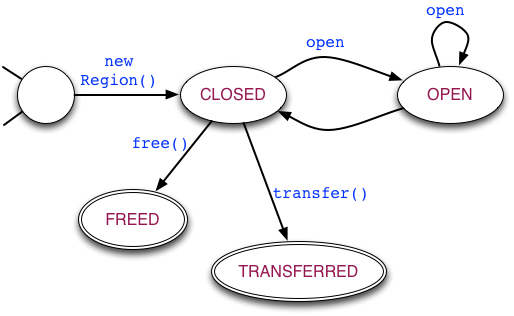
\includegraphics[scale=0.45]{region-fsm.png}
\caption{The lifetime of a dynamic (transferable) region in \name}
\label{fig:region-fsm}
\end{figure}

A transferable region starts its lifetime in a \emph{closed} state,
when it is created through \C{new Region} expresion. \name provides
\C{open} lexical construct to \emph{open} a transferable region as an
allocation context, and to access its root object:
\begin{codejava}
  Region<string> rgn = new Region<List<String>>
                        (() => new List<String>());
  open rgn as R0 withroot strList {
    strList.addAtHead("World");
    strList.addAtHead("Hello");
  }
  rgn.transfer();
\end{codejava}
In the above code, the \C{open} lexical block performs the
following operations: (a). It opens the transferable region handled by
\C{rgn} for allocation (i.e., makes it the current allocation
context), (b). assigns the identifier \C{R0} to the open region, and
(c). sets the newly introduced local variable (\C{strList}) to refer
to its root object (a list of strings). As Fig.~\ref{fig:region-fsm}
indicates, it is not possible to open a region that is already
transferred/freed. The fact that \C{rgn} is open within the block
therefore guarantees that it is not yet transferred/freed, and that
dereferencing \C{strList} within the block is safe. The end of
\C{open} block marks the return of transferable region to the closed
state.  While closed, the region is eligible to be transferred to a
downstream actor, or to be freed.  An actor that receives the
transferable region, receives it in the closed state. It can then
reopen the received region to read its contents, possibly add more
data and transfer it to another actor, or free the region. 

\name lets stack regions to be used as working memory while operating
with the data stored in a transferable region. Consider the following
code, for instance\footnote{For brevity, we drop \C{as} part of the
\C{open} expression whenever there is no need to assign a static
identifier for the open region.}:
\begin{codejava}
void onReceive(Region<List<String>> rgn)
  open rgn withroot strList {
    letregion R1 {
      String s = "";
      ListIterator<String> i = strList.listIterator();
      while(i.hasNext()) {
        s += i.getNext();
      }
      print s; //prints "HelloWorld"
    }
  }
  rgn.free();
}
\end{codejava}
The stack region \C{R1} is being used in the above code to provide
working memory to work with the objects of transferable region
\C{rgn}. Since a transferable region cannot be transferred/freed while
it is still open (Fig~\ref{fig:region-fsm}), \C{rgn} is guaranteed to
outlive the stack region \C{R1} in the above code, making it safe for
the later to contain references to the former. \name therefore allows
such references.

% The design decisions reflected above, \emph{viz.}, to ascribe a root
% object to every transferable region, to make use of a higher-order
% argument to initialize the root object, and to require that a region
% be explictly opened in a lexical block for allocations, were made to
% reflect the message semantics of transferable regions, to promote
% uniform style of programming with different kinds of regions, and to
% precisely state and enforce the safety guarantees offered by \name's
% region type system (\S~\ref{sec:type-system}).

As evident in the above examples, the safety of memory accesses in
\name is now subject to the condition that every transferable region
correctly follows the state transition discipline shown
in Fig.~\ref{fig:region-fsm}. If this is
guaranteed, then \name's region type system statically guarantees the
safety of all memory accesses. In other words, the type system reduces
the problem of ensuring memory safety in \name programs to the problem
of enforcing the state transition discipline for transferable regions.

In \name, this enforcement is done at runtime by explicitly keeping
track of the \emph{current state} for $\RgnZ$ objects, and
checking the validity of every open, transfer, or free operation
and throwing an exception if it is invalid.
The challenge in enforcing this discipline statically is that transferable regions
are first-class objects. Hence, the program can create multiple aliases for
the same region, \eg, open it via one alias and free it via another.
Typestate verification in the presence of aliases is hard.
The checking can be done statically by preventing the creation of aliases using, \eg, linear types
or unique types. However, this would be quite restrictive, in terms of expressiveness.

\name chooses a reasonable tradeoff. Regions are coarse-grained objects, manipulated relatively infrequently,
in comparison to manipulations of the fine-grained objects that reside inside regions. Hence, the programmer burden
as well as the runtime overhead of checking the region's state transition discipline is acceptable.

\begin{figure}[t!]
\begin{numcodejava}
class SelectVertex<TIn extends Cloneable, TOut> {
  Func<TIn, TOut> mapFn;
  Func<TIn, bool> whereFn;
  SelectVertex(Func<TIn, TOut> mapFn, 
               Func<TIn, bool> whereFn) {
    this.mapFn = mapFn;
    this.whereFn = whereFn;
  }
  void onReceive(Region<List<TIn>> inRgn) {
    Func<void,List<TOut>> f = 
        () => new List<TOut>();
    Region<List<TOut>> outRgn =
        new Region<List<TOut>>(f);
    open inRgn withroot inMsg {
      letregion R0 {
        ListIterator<TIn> iter = 
            inMsg.listIterator();
        while (iter.hasNext()) {
          TIn inp = iter.getNext();
          if (!this.whereFn(inp)) continue;
          openalloc outRgn withroot outMsg {
            TOut outp = this.mapFn(inp.clone());
            outMsg.add(outp);
          }
        }
      }
    }
    inRgn.free();
    outRgn.transfer();
  }
}
\end{numcodejava}
\caption{\C{SELECT} dataflow operator written in \name}
\label{fig:naiad-ex}
\end{figure}


\subsection{An Example}

Fig~\ref{fig:naiad-ex} shows \C{SelectVertex} class, which is a
straightforward implementation of the \C{SELECT} dataflow operator.
\C{SelectVertex} implements \C{onReceive} method, which is called by
the run-time when a message from an upstream actor is ready to be
delivered. A message is usually a sequence of tuples (e.g., key-value
pairs) wrapped inside a transferable region (\C{inRgn}).
\C{SelectVertex} opens its input region \C{inRgn} (line 16), iterates
through the sequence, filtering the input tuples that meet the
selection criterion of the \C{whereFn} (line 19), and applying the
\C{mapFn} to map the selected input tuples to output (line 22).
Observe that the iterator is allocated in the temporary (stack) region
\C{R0} that lives just long enough.  Functions \C{mapFn} and
\C{whereFn} are defined by the users of the dataflow system, hence
they are called \emph{user-defined functions}.  Unlike dataflow system
builders, users are oblivious of regions, hence user-defined functions
are expected to not contain explicit region annotations. While
\C{whereFn} defines the selection criterion that the user is
interested in (e.g: \C{age $\ge$ 18}), \C{mapFn} can either project
attributes of its input tuple amounting to type \C{TOut}, or can
create and return a new \C{TOut} object. Note that, unlike \C{inRgn},
the output transferable region (\C{outRgn}) was opened for allocation
and the \C{mapFn} is applied under this allocation context. Also note
that the input tuple is cloned under this allocation context.
Consequently, the result (\C{outp}) of applying the \C{mapFn} (line
22), which is subsequently added to \C{outMsg}, is guaranteed to be in
the \C{outRgn} regardless of the semantics of \C{mapFn}. On the other
hand, if the input tuple is not cloned (i.e., \C{inp} instead of
\C{inp.clone()} on line 22) and the \C{mapFn} simply projects its
input, then \C{outp} refers to an object inside \C{inp}, which no
longer exists when the \C{outRgn} is transferred to a downstream
actor. Therefore, if \C{mapFn} is applied over \C{inp} instead of
\C{inp.clone()}, then it better be a function that creates and returns
a new \C{TOut} object. Under such scenario, the region type of
\C{SelectVertex.mapFn} should be precise enough to prevent it from
being assigned a function (line 6) that simply returns its input.
Fortunately, \name's region type system (\S~\ref{sec:type-system}) is
capable of capturing such nuances in the type of
\C{SelectVertex.mapFn}. Furthermore, the type can be automatically
inferred by \name's region type inference
(\S~\ref{sec:type-inference}), which can peform the above non-trivial
reasoning on behalf of the programmer.



\section{\fbname}
\label{sec:type-system}

The purpose of \name's region type system is to enforce the key
invariant required for memory safety, namely that an object $o_1$ in a
region $R_1$ contains a reference to an object $o_2$ in $R_2$, only if
$R_2$ is guaranteed to outlive $R_1$. Intuitively, the invariant can
be enforced by (a). tracking \emph{outlives} relationships between
various regions in the program (b). tagging the C\# type of every
object in the program with its allocation region, and (c).  ensuring
that, when a reference is created, its target object ($o_2$) is
allocated in a region that is known to be in outlives relationship
with the object containing the reference. We now formally develop this
intuition via \fbname, our explicitly typed core language (with region
types) that incorporates the features introduced in the previous
section. \fbname builds on the Featherweight Generic Java
(FGJ)~\cite{fgj} formalism, and reuses notations and various
definitions from~\cite{fgj}, such as the definition of type
well-formedness for the core (region-free) language. 

% In this section, we formally develop \fbname, a language that
% incorporates the features introduced in the previous section, as well
% as its type system, building on the Featherweight Generic Java
% (FGJ)~\cite{fgj} formalism.  Our development reuses notations and
% various definitions from~\cite{fgj}, such as the definition of type
% well-formedness for the core (region-free) language, which are
% elaborated further in the supplement~\cite{techrep}.

\subsection{Syntax}
\label{sec:fb-syntax}

\begin{figure*}[t!]
%
\begin{smathpar}
\renewcommand{\arraystretch}{1.2}
\begin{array}{lclcl} 
\multicolumn{5}{c}{
  {\rgn} \in \mathtt{Static \; region \; ids} \qquad
  {\rho} \in \mathtt{Region \; variables} \qquad
  {\tyvar, \tyvarb} \in \mathtt{Type \; variables} \qquad
  {m} \in \mathtt{Method \; names} \qquad
  {x,y,f} \in \mathtt{Variables \; and \; fields} }\\
cn & \in & \M{Class \; names} & \coloneqq & \ObjZ \ALT \RgnZ \ALT A \ALT B\\
     \fgjN & \in & \M{FGJ \; class \; types} & \coloneqq & cn\inang{\tbar}\\
T  & \in & \M{FGJ \; types} & \coloneqq & \tyvar \ALT  \fgjN \ALT \unitZ
     \ALT \bar{T} \rightarrow T \\
\fbN  & \in & \M{Region-annotated \; class \; types} & \coloneqq & 
     cn\inang{\tbar}\inang{\rbar} \\
\tau &\in& \M{types} & \coloneqq & T@\rgn  
      \ALT \fbN \ALT \unitZ 
      \ALT \inang{\rhobar \,|\, \phi}\bar{\tau}
      \xrightarrow{\rgn} \tau \\
C  & \in & \M{Class \; definitions} & \coloneqq & 
     \C{class} \; cn\inang{\bar{\tyvar} \extends \bar{\fgjN}} 
                    \inang{\rhobar \,|\, \phi}\extends \fbN 
                    \{\bar{\tau} \; \bar{f};\; \bar{d}\}\;\\
%k  & \in & \M{Constructors} & \coloneqq & 
%     cn(\bar{\tau} \; \bar{x})\{\C{super}(\bar{x}); \;
%                                \C{this}.\bar{f}\,=\,\bar{x};\}\\
d  & \in & \M{Methods} & \coloneqq & 
     \tau \; m\inang{\rhobar \,|\, \phi} (\taubar \; \xbar)
     \{\C{return}\;e;\}\\
\phi,\phicx &\in& \M{Region\;constraints} & \coloneqq & true 
      \ALT \rho \outlives \rho \ALT \rho = \rho \ALT \phi \conj \phi\\
e  & \in & \M{Expressions} & \coloneqq & \unitval \ALT x \ALT e.f 
     \ALT e.m\inang{\rbar}(\ebar) \ALT \C{new}\;\fbN(\ebar)
     \ALT \lambdaexp{\rgn}{\rhobar \,|\, \phi}
                    {\xbar:\taubar} {e}
           \ALT e\inang{\rbar}(\bar{e})\\
   & & & & \ALT \letexp{x}{e}{e} \ALT \letregion{\rho}{e} 
           \ALT \open{x}{\rgn}{y}{e} \\
\end{array}
\end{smathpar}

\caption{\fbname: Syntax}
\label{fig:fb-syntax}
\end{figure*}


Fig~\ref{fig:fb-syntax} describes the syntax of \fbname (\FB). Class
types in \FB are region-annotated variants of class types in FGJ (also
called \emph{core types}). This correspondence is reflected in the
$T@\rgn$ syntax of a region type, which is the simplest form of a
region type describing an object of core type $T$ contained in a
region $\rgn$. We let $\rgn$ range over static identifiers of regions
in \FB. The only unboxed value in \FB is $\unitval$ of type \unitZ.
Rest are objects.

\FB extends FGJ's expression language with assignments, local variable
declarations (via \C{let} expressions), region constructs
(\C{letregion} and \C{open}), lambda abstraction
($\lambdaexp{...}{\xbar : \taubar}{e}$) and application
($e\inang{...}(\bar{e})$) expressions. Assignments and region
constructs, which are statements in \name, are treated as effectful
expressions in \FB. Lambda abstraction and application expressions are
to define and apply anonymous functions. Modulo the angle braces
(whose presence will be justified later), these expressions are
uncurried variants of the corresponding expressions from System F.
Since FGJ formalism does not include higher-order functions, we extend
the syntactic class (\C{T}) of FGJ types with an (uncurried) arrow
type.

Class definitions in \FB extend FGJ's with region parameters
($\rho$). Informally, region variables ($\rho$) are to region
identifiers ($\rgn$) as type variables ($a$) are to core types ($T$);
they can be instantiated with region identifiers, as needed. A class
in \FB is necessarily parameterized over the allocation region of its
objects. We use $\rho^a$ to denote this parameter, and often refer to
it as \emph{class}'s allocation region, although it is really the
allocation region of its objects. An Object in \FB can contain fields
referring to objects allocated in regions ($\rhobar$) other than its
own allocation region ($\rhoalloc$), provided that the former outlive
the later (i.e., $\rhobar \outlives \rho$). In such cases, the
definition of object's class needs to be parametric over allocation
regions of its fields (i.e., their classes). Furthermore, the
constraint that such regions must outlive the allocation region of the
class needs to be made explicit in the definition. For instance, a
\C{Pair} object allocated in a region ${\rhoalloc}$ can have its first
component coming from ${\rho_1}$ and second from $\rho_2$, where all
the $\rho$'s are distinct, and $\rho_1, \rho_2$ outlive
$\rhoalloc$. The corresponding definition of the \C{Pair} class is as
follows(The symbol $\extends$ should be read \emph{extends}):  
\begin{codejava}[mathescape=true]
class Pair<a $\extends$ Object, b $\extends$ Object>
          <$\rho^a, \rho_1, \rho_2 \,|\, \rho_1 \outlives \rho^a \conj \rho_2 \outlives \rho^a$> $\extends$ Object<$\rho^a$>
           {
  a@$\rho_1$ fst; 
  b@$\rho_2$ snd;
  Pair(a@$\rho_1$ fst, b@$\rho_2$ snd) {
    super(); 
    this.fst = fst; 
    this.snd = snd;
  }
  a@$\rho_1$ getFst() {
    return this.fst;
  }
}
\end{codejava}
To construct objects of the \C{Pair} class, its type and region
parameters need to be instantiated with core types ($T$) and concrete
region identifiers ($\rgn$), respectively. For example:
\begin{codejava}
letregion $\rgn_0$ {
  Object<$\rgn_0$> snd = new Object<$\rgn_0$>();
  letregion $\rgn_1$ {
    Object<$\rgn_1$> fst = new Object<$\rgn_1$>();
    let p = new Pair<Object,Object><$\rgn_1$,$\rgn_0$,$\rgn_1$>
                  (fst,snd);
  }
}
\end{codejava}
In the above code, the instantiation of $\rhoalloc$ and $\rho_1$ with
$\rgn_0$, and $\rho_2$ with $\rgn_1$ is allowed because (a) $\rgn_0$
and $\rgn_1$ are live during the instantation, and (b). $\rgn_0
\outlives \rgn_1$ and $\rgn_1 \outlives \rgn_1$ (since outlives is
reflexive). Observe that the region type of \C{p} conveys
the fact that (a). it is allocated in region $\rgn_1$, and (b). it
holds references to objects allocated in region $\rgn_0$ and $\rgn_1$.
In contrast, if we choose to allocate the \C{snd} object also in
$\rgn_1$, the region type of \C{p} would be
\C{Pair<\ObjZ,\ObjZ><$\rgn_1$,$\rgn_1$,$\rgn_1$>}, which we abbreviate
as \C{Pair<\ObjZ,\ObjZ>@$\rgn_1$}\footnote{In general, we treat
$B\inang{\tbar}@\rgn$ as an abbreviation of
$B\inang{\tbar}\inang{\rbar}$}. The $\ObjZ$ class in \FB has no
fields, hence its region type is of form $\ObjZ@\rgn$.
% In general, the \C{@} notation in a
% region type of an object \C{x} highlights that
% \C{x}, and all the objects reachable from \C{x} via references are
% allocated in a single region. We say that \C{x} is \emph{contained} in
% the region. The $\ObjZ$ class in \FB contains no references to other
% objects, hence its objects are always contained in their allocation
% region. Their region type is $\ObjZ\inang{\rgn}$ (or equivalently,
% $\ObjZ@\rgn$), for some region $\rgn$.

% Note that when a generic class definition in FGJ is lifted to a
% region-polymorphic definition in \FB, it nonetheless remains generic
% with respect to core types. We say that the class is now a
% region-polymorphic generic class. Region parameterization of a class
% in \FB is independent of its parameterization over core types; they
% are not conflated to make the class parametric over region types. For
% instance, following is the region-polymorphic definition of a generic
% \C{Pair} class (The symbol $\extends$ should be read \emph{extends}):

% When objects of a class are allocated in a region $\rgn$, it means
% that the class's constructor is run with $\rgn$ as its allocation
% context. Every class definition in \FB is necessarily polymorphic with
% respect to the allocation region of its objects, i.e., the allocation
% context of its constructor. We adopt a convention that requires the
% allocation region parameter (denoted $\rho^a$) to be the first region
% parameter of a class.  Besides the allocation region of its objects,
% \C{Pair} class is also parametric over the regions its first and
% second elements are allocated in. References between objects allocated
% in different regions are only allowed if the referred object is
% guaranteed to outlive the referring object. In case of \C{Pair} class,
% this means that allocation regions ($\rho_1$ and $\rho_2$) of both
% objects that make up the pair must outlive the allocation region
% ($\rho^a$) of the \C{Pair} object. Such conditions over region
% parameters of a class need to be recorded in its header as region
% constraints ($\phi$) in order for the class to be judged well-formed
% by the type system (Fig.~\ref{fig:fb-morewfrules}). 

%%An object \emph{allocated} in a region $\rgn$ contains its spine in
%%$\rgn$, but can refer to objects allocated in other regions.  On the
%%other hand,

% \FB's $\RgnZ$ objects, like $\ObjZ$ objects, have region type of form
% $\RgnZ\inang{\rgn}$. However, unlike the $\rgn$ in
% $\ObjZ\inang{\rgn}$, $\rgn$ in $\RgnZ\inang{\rgn}$ cannot be any
% region. Recall that $\RgnZ$ objects have special semantics in \name -
% they act as handlers to transferable regions.  Constructing a new
% $\RgnZ$ object entails the creation of a new transferable region, and
% it is in this region that the new object is allocated in. It follows
% that $\rgn$ in $\RgnZ\inang{\rgn}$ should be the static identifier of
% the new transferable region. But, static identifiers for transferable
% regions are introduced only when such regions are opened for
% allocation via \C{open} expression. What, then, should be the region
% type of a \C{new Region} expression?

% \FB resolves this problem by existentially quantifying the allocation
% region of $\RgnZ$ objects when they are created. In other words, the
% type of \C{new Region} expression in \FB is
% $\exists\rho.\RgnZ\inang{\rho}$. Existential quantification in the
% type captures the fact that there now exists a transferable region
% containing the newly constructed $\RgnZ$ object. Elimination of
% existential quantification is facilitated by the \C{open} expression,
% which opens the transferable region and assigns it an identifier
% ($\rgn$).  Within the scope of \C{open}, the transferable region is
% identified with $\rgn$, allowing its handler to instantiate the
% existentially bound region variable with $\rgn$, and assume the type
% of $\RgnZ\inang{\rgn}$.

Like classes, methods can also exhibit qualified region polymorphism.
A method definition in \FB is necessarily polymorphic over its
allocation context (Sec.~\ref{sec:alloc-ctxt}), and optionally
polymorphic with respect to the regions containing its arguments.
Region parameters, like those on classes, are qualified with
constraints ($\phi$).
% Region parameters on the methods, like those on classes, are
% accompanied by constraints ($\phi$) capturing the conditions that the
% parameters need to satisfy for the method to be considered well-formed
% (Fig.~\ref{fig:fb-morewfrules}). Allocation context (usually $\rho^a$
% or $\rho^a_m$) is the first and inevitable region parameter of every
% method in \FB. 
Note that if a method is not intended to be polymorphic with respect
to its allocation context (for example, if its allocation context
needs to be same as the allocation region of its \emph{this}
argument), then the required monomorphism can be captured as an
equality constraint in $\phi$.  

% Like methods, functions can also be region-polymorphic. 
% A lambda expression defines a region-polymorphic
% multi-argument function closure parameterized over function's
% allocation context parameter. 
The angle braces in the lambda expression ($\inang{\rho^a\rhobar \,|\,
\phi}$) serve the same purpose as they do in a method definition - to
capture region parameters along with their constraints. Region
parameters also appear in the arrow type of the lambda expression 
($\inang{\rhoalloc\rhobar \,|\, \phi}\bar{\tau} \xrightarrow{\rgn}
\tau$) at the prenex position, similar to ML type schemes. However,
unlike ML, we don't distinguish between types and type schemes; any of
the $\tau$'s in the arrow type can themselves be region-parametric
arrow types. Like with methods, region parameters on functions can be
instantiated when they are applied.
% In this respect, our region type system is more like
% System F's type system, which admits higher-rank parametric
% polymorphism. Like System F, \FB provides a region instantiation
% expression ($e\inang{\ralloc\rbar}$), and a region generalization
% expression ($\Lambdaexp{\rhoalloc\rhobar \,|\, \phi}{e}$) to
% instantiate and generalize region variables. 

A lambda expression creates a closure, which can escape the
context in which it is created. It is therefore important to keep track of
the region in which a closure is allocated in order to avoid unsafe
dereferences. The $\rgn$ annotation above the arrow in the arrow
type denotes the allocation region of the corresponding closure. Note
that it is important to distinguish between the allocation context
argument ($\rhoalloc$) of a function and the allocation region
($\rgn$) of its closure. In \name, the later corresponds to the region where
a \C{Func} object is allocated, while the former corresponds to the
region where it is applied ($e\inang{\ralloc\rbar}(\bar{e})$). 
% For instance, in the following example:
% \begin{codejava}
% letregion $\rgn$ {
%   let f = $\lambda{\inang{\rho^a}}$().$\,$new Object$\inang{\rho^a}$() 
%   in f
% }
% \end{codejava}
% The type of \C{f} is $\inang{\rho^a}\unitZ \xrightarrow{\rgn}
% \ObjZ\inang{\rho^a}$, coveying that (a). \C{f}'s closure is allocated
% in $\rgn$, and (b). when executed under an allocation context
% $\rho^a$, the closure returns an object allocated in $\rho^a$.

\begin{figure*}[t]
%
\textbf{Auxiliary Definitions} \\
\begin{minipage}{1.75in}
\begin{smathpar}
\begin{array}{lcl}
  allocRgn(A\inang{\rhoalloc\rhobar}\inang{\tbar}) & = & \rhoalloc\\
  bound_{\Delta}(\alpha) & = & \Delta(\alpha)\\
  bound_{\Delta}(N) & = & N\\
\end{array}
\end{smathpar}
\end{minipage}
%
\begin{minipage}{1.8in}
\begin{smathpar}
\begin{array}{c}
\renewcommand*{\arraystretch}{1.2}
\RULE
  {
    \\
    B \in \{\ObjZ,\RgnZ\}
  }
  {
    fields(B\inang{\ralloc\rbar}\inang{\tbar}) \;=\; \bullet
  }
\end{array}
\end{smathpar}
\end{minipage}
%
\begin{minipage}{3in}
\begin{smathpar}
\begin{array}{c}
\renewcommand*{\arraystretch}{1.2}
\RULE
  {
    CT(B) = \headerOf{B}\{\bar{\tau^f}\;\bar{f};\,...\}\\
    \substFn = [\rbar/\rhobar, \ralloc/\rhoalloc, \tbar/\bar{\alpha}] \qquad 
    fields(\substFn(N)) = \bar{\tau^g}\;\bar{g}
  }
  {
    fields(B\inang{\ralloc\rbar}\inang{\tbar}) \;=\;
      \bar{\tau^g}\,\bar{g},\,\substFn(\bar{\tau^f})\,\bar{f}
  }
\end{array}
\end{smathpar}
\end{minipage}
%
\bigskip

\begin{minipage}{3.75in}
\begin{smathpar}
\begin{array}{c}
\renewcommand*{\arraystretch}{1.2}
\RULE
  {
    CT(B) = \headerOf{B}\{\bar{\tau^f}\;\bar{f};\,k\;\bar{d}\}\\
    \tau^2 \; m\mang (\bar{\tau^1}\;\bar{x})\{...\} \in \bar{d} \qquad
    \substFn = [\rbar/\rhobar, \ralloc/\rhoalloc, \tbar/\bar{\alpha}]
  }
  {
    mtype (m,B\inang{\ralloc\rbar}\inang{\tbar}) \;=\;
    \substFn(\mang\bar{\tau^1} \rightarrow \tau^2)
  }
\end{array}
\end{smathpar}
\end{minipage}
%
\begin{minipage}{3in}
\begin{smathpar}
\begin{array}{c}
\renewcommand*{\arraystretch}{1.2}
\RULE
  {
    CT(B) = \headerOf{B}\{\bar{\tau^f}\;\bar{f};\,k\;\bar{d}\}\\
    m \notin \bar{d} \qquad 
    \substFn = [\rbar/\rhobar, \ralloc/\rhoalloc, \tbar/\bar{\alpha}]
  }
  {
    mtype (m,B\inang{\ralloc\rbar}\inang{\tbar}) \;=\;
    mtype (m, \substFn(N))
  }
\end{array}
\end{smathpar}
\end{minipage}
%
\bigskip
\begin{smathpar}
\A \;=\; (\subtypcx)
\end{smathpar}
%
\bigskip

\textbf{Subtyping}  \; \fbox
  {\(\subtyp{\A}{\tau_1}{\tau_2}\)}\\

%
\begin{minipage}{1in}
\begin{smathpar}
\begin{array}{c}
\renewcommand*{\arraystretch}{1.2}
\RULE
  {
    \\
  }
  {
    \subtyp{\A}{\tau}{\tau}
  }
\end{array}
\end{smathpar}
\end{minipage}
%
\begin{minipage}{1.2in}
\begin{smathpar}
\begin{array}{c}
\renewcommand*{\arraystretch}{1.2}
\RULE
  {
    \\
  }
  {
    \subtyp{\A}{\tyvar @\rho}{\aenv(\tyvar) @\rho}
  }
\end{array}
\end{smathpar}
\end{minipage}
%
\begin{minipage}{2in}
\begin{smathpar}
\begin{array}{c}
\renewcommand*{\arraystretch}{1.2}
\RULE
  {
    \subtyp{\A}{\tau_1}{\tau_2}\qquad
    \subtyp{\A}{\tau_2}{\tau_3}
  }
  {
    \subtyp{\A}{\tau_1}{\tau_3}
  }
\end{array}
\end{smathpar}
\end{minipage}
%
\begin{minipage}{1.5in}
\begin{smathpar}
\begin{array}{c}
\renewcommand*{\arraystretch}{1.2}
\RULE
  {
    \\
  }
  {
    \subtyp{\A}{\exists\rho.\tau}{\exists\rho'.[\rho'/\rho]\tau}
  }
\end{array}
\end{smathpar}
\end{minipage}
%
\bigskip
\begin{minipage}{1.5in}
\begin{smathpar}
\begin{array}{c}
\renewcommand*{\arraystretch}{1.2}
\RULE
  { }
  { }
\end{array}
\end{smathpar}
\end{minipage}
%
\begin{minipage}{3.5in}
\begin{smathpar}
\begin{array}{c}
\renewcommand*{\arraystretch}{1.2}
\RULE
  {
    CT(B) = \headerOf{B}\{\bar{\tau^f}\;\bar{f};\,k\;\bar{d}\}\\
    \tywf{\A}{B\inang{\pi^a\bar{\pi}\inang{\taubar}}}\qquad
    \substFn = [\rbar/\rhobar, \ralloc/\rhoalloc, \tbar/\bar{\tyvar}] \qquad 
    \tywf{\A}{\substFn(\fbN)}
    \
  }
  {
    \subtyp{\A}{B\inang{\pi^a\bar{\pi}\inang{\taubar}}}{\substFn(\fbN)}
  }
\end{array}
\end{smathpar}
\end{minipage}
%

%
\bigskip

\textbf{Well-formedness}  \; \fbox
  {\(\tywf{\A}{\tau}, \spc 
     \tywf{\A}{\phi}\)}\\

%
\begin{minipage}{1.25in}
\begin{smathpar}
\begin{array}{c}
\renewcommand*{\arraystretch}{1.2}
\RULE
  {
    \\
    \\
    \rgn \in \A.\rhoenv
  }
  {
    \tywf{\A}{\ObjZ\inang{\rgn}}
  }
\end{array}
\end{smathpar}
\end{minipage}
% %
% \begin{minipage}{1.5in}
% \begin{smathpar}
% \begin{array}{c}
% \renewcommand*{\arraystretch}{1.2}
% \RULE
%   {
%     \rgn \in \A.\rhoenv\\
%     \fgjtywf{\A.\aenv}{\RgnZ\inang{T}}
%   }
%   {
%     \tywf{\A}{\RgnZ\inang{\rgn}\inang{T}}
%   }
% \end{array}
% \end{smathpar}
% \end{minipage}
% %
% \begin{minipage}{1.5in}
% \begin{smathpar}
% \begin{array}{c}
% \renewcommand*{\arraystretch}{1.2}
% \RULE
%   {
%     \fgjtywf{\A.\aenv}{\RgnZ\inang{T}}
%   }
%   {
%     \tywf{\A}{\exists\rho.\RgnZ\inang{\rho}\inang{T}}
%   }
% \end{array}
% \end{smathpar}
% \end{minipage}
%
\begin{minipage}{2.75in}
\begin{smathpar}
\begin{array}{c}
\renewcommand*{\arraystretch}{1.2}
\RULE
  {
    \rgn \in \A.\rhoenv \spc
    \{\rhoalloc,\rhobar\} \notin \A.\rhoenv \\
    \A' = (\A.\rhoset, \A.\rhoenv \cup \{\rhoalloc,\rhobar\}, 
           \A.\aenv, \A.\phicx \conj \phi) \\
    \tywf{\A'.\rhoenv}{\phi}\spc 
    \tywf{\A'}{\bar{\tau^1}} \spc
    \tywf{\A'}{\tau^2}
  }
  {
    \tywf{\A}{\inang{\rhoalloc\rhobar \,|\, \phi}
              \bar{\tau^1} \xrightarrow{\rgn} \tau^2}
  }
\end{array}
\end{smathpar}
\end{minipage}
%
\begin{minipage}{1.5in}
\begin{smathpar}
\begin{array}{c}
\renewcommand*{\arraystretch}{1.2}
\RULE
  { 
    \\
    \\
    \fgjtywf{\A.\aenv}{T}
  }
  {
    \tywf{\A}{\RgnZ\inang{T}\inang{\rgn}}
  }
\end{array}
\end{smathpar}
\end{minipage}
%
\begin{minipage}{1in}
\begin{smathpar}
\begin{array}{c}
\renewcommand*{\arraystretch}{1.2}
\RULE
  {
    \\
    \\
    \rho_0,\rho_1 \in \rhoenv
  }
  {
    \tywf{\rhoenv}{\rho_0 \outlives \rho_1}
  }
\end{array}
\end{smathpar}
\end{minipage}
%

%
\begin{minipage}{3.5in}
\begin{smathpar}
\begin{array}{c}
\renewcommand*{\arraystretch}{1.2}
\RULE
  {
    CT(B) = \headerOf{B}\{...\}\spc
    \ralloc,\rbar \in \A.\rhoenv \\
    \fgjtywf{\A.\aenv}{B\inang{\tbar}}\spc
    \substFn = [\rbar/\rhobar, \ralloc/\rhoalloc, \tbar/\bar{\tyvar}] \spc
    \isvalid{\A.\phicx}{\substFn(\phi)}
  }
  {
    \tywf{\A}{B\inang{\ralloc\rbar}\inang{\tbar}}
  }
\end{array}
\end{smathpar}
\end{minipage}
%
\begin{minipage}{1.65in}
\begin{smathpar}
\begin{array}{c}
\renewcommand*{\arraystretch}{1.2}
\RULE
  {
    \fgjtywf{\A.\aenv}{T}\spc
    \ralloc \in \A.\rhoenv\\
    \fgjsubtyp{\A.\aenv}{T}{\ObjZ}\spc
  }
  {
    \tywf{\A}{T@\ralloc}
  }
\end{array}
\end{smathpar}
\end{minipage}
%
\begin{minipage}{0.75in}
\begin{smathpar}
\begin{array}{c}
\renewcommand*{\arraystretch}{1.2}
\RULE
  {
    \tywf{\rhoenv}{\phi_0} \\ \tywf{\rhoenv}{\phi_1}
  }
  {
    \tywf{\rhoenv}{\phi_0 \wedge \phi_1}
  }
\end{array}
\end{smathpar}
\end{minipage}

%
\bigskip
\caption{Static semantics of {\sc Featherweight} \name}
\label{fig:fb-syntax}
\end{figure*}

\subsection{Types and Well-formedness}

Static semantics of \fbname is defined by the rules to establish
well-formedness of region types and region constraints, check
subtyping between a pair of region types, and type-check expressions
against region types. Fig.~\ref{fig:fb-staticsem} contains an
illustrative subset of such rules\footnote{The full formal development
can be found in our technical report~\cite{techrep}}, along with some
auxiliary definitions. The judgments defined by these rules make use
of a context ($\A$), which is a tuple of:
\begin{itemize}
\item A set ($\rhoenv \in 2^\rgn$) of static identifiers of regions
that are estimated to be live,
\item A finite map ($\aenv \in \tyvar \mapsto \fgjN$) of type
variables to their bounds\footnote{A bound of a type variable
($\tyvar$) in FGJ~\cite{fgj} is the class ($\fgjN$) that type variable
was declared to extend.  The map $\tyvar \mapsto \fgjN$ is denoted
$\Delta$ in FGJ formalism}, and
\item A constraint formula ($\phicx$) that captures the outlives
constraints on regions in $\rhoenv$.
\end{itemize}
The context for the expression typing judgment also includes:
\begin{itemize}
\item A type environment ($\env \in x \mapsto \tau$) that contains the
type bindings for variables in scope, and 
\item The static identifier ($\rgn^a$) of the allocation context for
the expression is being type-checked.  
\end{itemize}

\begin{figure}

\begin{codejava}
class Region<a $\extends$ Object><${\rhoalloc}$> $\extends$ Object<$\rhoalloc$>{
  <${\rho}$>unit$\xrightarrow{\rhoalloc}$a@$\rho$ thunk;
  Region(<${\rho}$>unit$\xrightarrow{\rhoalloc}$a@$\rho$ thunk) {
    super(); 
    this.thunk = thunk;
  }
  unit transfer$\inang{\rho}$(unit u) {
    return u;
  }
}
\end{codejava}

\caption{The stub used for $\RgnZ$ class}
\label{fig:region-stub}
\end{figure}

\noindent The well-formedness judgment on region types
($\tywf{\A}{\tau}$) makes use of the well-formedness and subtyping
judgments on core types \footnote{We use a double-piped turnstile
($\Vdash$) for judgments in FGJ~\cite{fgj}, and a simple turnstile
($\vdash$) for those in \FB.}. All judgments are implicitly
parameterized on a class table ($CT \in cn \mapsto D$) that maps class
names to their definitions in \FB. For judgments in FGJ, we use a
class table that maps class names to their region-erased definitions.
We denote the region-erased class table as ($\absof{CT}$). The precise
semantics of region erasure ($\absof{\cdot}$) are defined
in~\cite{techrep}, but it can be understood as an operation that
erases region annotations on types. The class table is assumed to bind
the name $\RgnZ$ to the stub shown in Fig.~\ref{fig:region-stub}.
This mostly eliminates the need to treat $\RgnZ$ objects, which double
up as transferable region handlers, as a special case in semantics.

The well-formedness rule for region instantiation in class types
($B\inang{\tbar}\inang{\ralloc\rbar}$) requires that the region-erased
(core) type be well-formed, instantiated regions be live, and that
they satisfy the constraints ($\phi$) imposed by the class on its
region parameters. The later is enforced by checking the validity of
$\phi$, with actual region arguments substituted\footnote{The notation
$[a/b](e)$ stands for "$a$ is substituted for $b$ in $e$"} for formal
region parameters, under the conditions ($\A.\phicx$) guaranteed by
the context. The semantics of this sequent is straightforward, and
follows directly from the properties of outlives and equality
relations. For any well-formed core type $T$, $T@\rgn$ is a
well-formed region type if $\rgn$ is a valid region. Well-formedness
of region constraints requires that the regions referred by the
constraints be live.

The subtype relation between region types of objects
($B\inang{\ralloc\rbar}\inang{\tbar}$) follows directly from the
subclass relation between their class types. Note that, in general, we
don't lift outlives relation between regions to subtype relation
between objects (of same core type) allocated in those regions. Such
lifting is unsound for the same reason as covariant/contravariant
subtyping between mutable references is unsound. However, we make a
special case for $\RgnZ$ objects: we allow $\RgnZ$ objects allocated
in any region to be considered as objects allocated in an eternal
region ($\toprgn$) that outlives every other region. This lets $\RgnZ$
objects escape the context they are created in (as required by the
\C{transfer} operation), and also facilitates data structures of
regions created in different contexts (for e.g., a list of $\RgnZ$
objects, whose root objects are of (core) type $T$, can be typed
$\C{List}\inang{\RgnZ\inang{T}}\inang{\rgn,\toprgn}$, where $\rgn$ is
the region where the spine of the list is allocated). As described in
\S\ref{sec:memory-safety}, runtime checks are used to prevent the
unsound subtyping rule on region objects from effecting the memory safety.
% \begin{smathpar}
% \begin{array}{c}
% \renewcommand*{\arraystretch}{1.1}
% \RULE
%   {
%     \isvalid{\A.\phicx}{\rgn_1 \outlives \rgn_2}
%   }
%   {
%     \subtyp{\A}{T@{\rgn_1}}{T@{\rgn_2}}
%   }
% \end{array}
% \end{smathpar}

The actual implementations of region-based memory management for \name
may choose to realize the $\toprgn$ as a garbage-collected region, but
this is not required. Our operational semantics
(\S\ref{sec:fb-opsem}), for example, does not even associate a region
with $\toprgn$, instead opting to allocate $\RgnZ$ objects in the same
transferable regions that they represent. Our type safety result
nonetheless guarantees memory safety in this implementation.

% Such a rule is unsound for it allows an object in a region ($\rgn_1$)
% to be treated as an object in a shorter living region ($\rgn_2
% \underlives \rgn_1$), thus allowing it to refer to shorter living
% objects in $\rgn_2$. The type system should prevent such unsafe
% references by restricting subtype relation to only those region types
% that are invariant in their allocation region. For instance, assuming
% that class $A$ is a subclass of $\ObjZ$ (as per FGJ), the subtype
% relation $A@\rgn <: \ObjZ@\rgn$ should be allowed, but not the
% relation $A@\rgn <: \ObjZ@\rgn'$, for any $\rgn' \neq \rgn$. \FB's
% type system enforces this not by restricting the subtype rule, but by
% constraining the subclass relation between region-annotated classes.
% In particular, it lets a class $A\inang{\rhoalloc}$ to be declared to
% extend $\ObjZ\inang{\rhoalloc}$, but never to extend
% $\ObjZ\inang{\rhoalloc_1}$, where $\rhoalloc_1 \neq \rhoalloc$. The
% well-formedness rule on class definitions (not shown) captures this
% restriction.

As expected, subtyping between arrow types is contravariant in
argument types and covariant in return types. It is also contravariant
in the region constraints that the region parameters have to satisfy.
For example, the type $\inang{\rhoalloc\rho} A@\rho \xrightarrow{\rgn}
\unitZ$ is a subtype of $\inang{\rhoalloc\rho \,|\, \rho =  \rhoalloc}
A@\rho \xrightarrow{\rgn} \unitZ$, for the former's precondition is
weaker than the later's. Finally, the subtyping is invariant with
respect to the allocation region ($\rgn$) of closures. 
% This subtype rule assumes that both arrow types have same set of
% region parameters.  However, this is not restrictive as (a). it is
% possible to add more region parameters to a function type and declare
% them to be equal to existing ones (as the arrow type above does), and
% (b). it is possible to rename region parameters by composing
% instantiation and generalization (big-lambda) expressions together.

The type rule for \C{letregion} expression requires that the static
identifier introduced by the expression be unique under the current
context (i.e., $\rgn \notin \rhoenv$). This condition is needed in
order to prevent the new region from incorrectly assuming any existing
outlives relationships on an eponymus region. Provided this is
satisfied, the expression ($e$) under \C{letregion} is then
type-checked against $\unitZ$ assuming that the new region is live
($\rgn \in \rhoenv$) and that it is outlived by all existing live
regions ($\rhoenv \outlives \rgn$).

Like the rule for \C{letregion}, the type rule for the \C{open}
expression requires that the static identifier ($\rgn$) introduced to
refer to the transferable region being opened be unique. However,
unlike the \C{letregion} rule, the rule for \C{open} does not
introduce any outlives relationship between the newly opened region
and any pre-existing region while checking the type of the expression
($e$) under \C{open}. This effectively preempts the possibility of any
references from objects inside the transferable region to those
outside. Environment ($\env$) is extended with binding for the type of
root object while type-checking $e$. 

The type rule for lamdba expression requires that its region
parameters ($\rhoalloc\rhobar$) be unique under the current context,
and that the constraints ($\phi$) over region parameters be
well-formed. The lambda-bound expression ($e$) is checked under an
extended type environment containing bindings for function's
arguments, assuming that region parameters are live, and that declared
constraints over region parameters hold. Note that the closure is
always allocated in the current allocation context ($\rgn^a$). This
prevents the closure from escaping the context in which it is created,
thus trivially ensuring the safety of any dereferences inside the
closure.

The type rule for the \C{new} expression is a straightforward
adaptation of corresponding FGJ rule to the the region type setting.

% The type rule for assignment expression ($e_1 := e_2$) ensures that a
% (local or instance) variable is only assigned objects of either the
% same type or a subtype. Recall that subtyping between region types is
% invariant with respect to the allocation regions of their objects. It
% follows that if a variable is declared to refer to objects in a region
% $\rgn$, then it is only ever assigned objects that allocated in
% $\rgn$. This prevents, for example, a temporary object allocated
% inside a stack region within a method from escaping the region's scope
% via an assignment to an instance variable.

\subsection{Operational Semantics and Type Safety}
\label{sec:fb-opsem}

Operational semantics of \fbname defines an evaluation relation
($\redsto$) over its expression language. In particular, the
evaluation gets stuck if an expression attempts to dereference a
pointer into a region that has either been deallocated or transferred.
On the other hand, if expression attempts to commit an operation on a
transferable region handler (a $\RgnZ$ object) that is not sanctioned
by the state transition discipline in Fig.~\ref{fig:region-fsm}, then
it is reduced to a value called $\invalidexn$. The accompanying
technical report~\cite{techrep} contains full operational semantics of
\fbname. 

To help state the type safety theorem, we extend \FB's expressions
with $\invalidexn$, and define the syntactic class of values:
\begin{smathpar}
\begin{array}{lclcl}
v & \in & \mathtt{values} & \coloneqq & \C{new}\; \fbN(\bar{v}) \ALT
\lambdaexp{\ralloc}{\rhoalloc\rhobar\,|\,\phi}{\taubar \; \xbar}{e}\\
\end{array}
\end{smathpar}
Type safety theorem is now stated thus:
\begin{theorem}
\emph{(\textbf{Type Safety})}
\label{thm:core-safety}
Let $\A_{\emptyset} = (\emptyset,\cdot,true)$ denote an empty context.
If $\hastyp{\A_{\emptyset}, \toprgn, \cdot}{e}{\tau}$, then either $e$
is a value, or $e \redsto \invalidexn$, or there exists an $e'$ such
that $e \redsto e'$ and $\hastyp{\A_{\emptyset}, \toprgn,
\cdot}{e'}{\tau}$.
\end{theorem}



% \appendix
% \section{Appendix Title}

% This is the text of the appendix, if you need one.

% We recommend abbrvnat bibliography style.

\bibliographystyle{abbrvnat}
\bibliography{catalyst}


\end{document}

